\section{Introduction}
\label{sec:introduction}

% state the learning objective 
\tab The objective of this laboratory assignment is to design a audio amplifier circuit keeping in mind that it must be cost efficient.
The circuit and its organization can be seen in Figure~\ref{fig:circuit}.
The values used in this circuit for the resistors and capacitor can be found in Table~\ref{tab:values}.

In Section~\ref{sec:analysis}, a theoretical analysis of the circuit is
presented. In Section~\ref{sec:simulation}, the circuit is analysed by
simulation, and the results are compared to the theoretical results obtained in
Section~\ref{sec:analysis}. The conclusions of this study are outlined in
Section~\ref{sec:conclusion}.
\\[1cm]
\begin{figure}[h] \centering
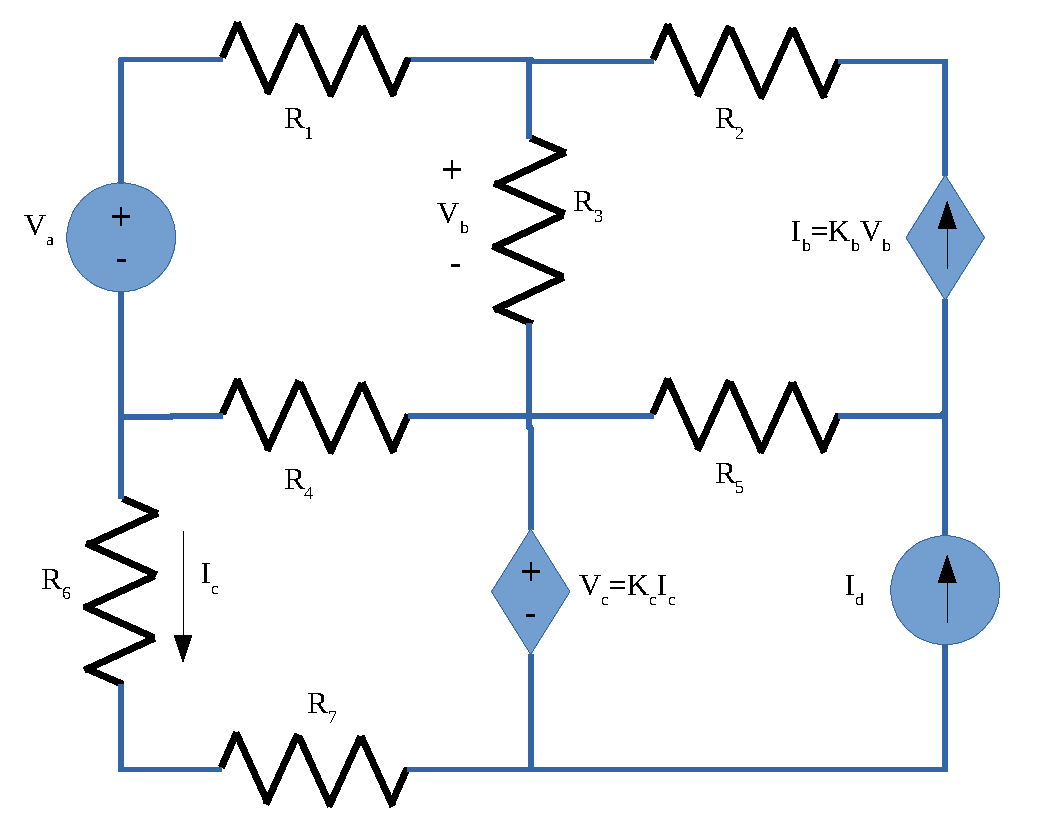
\includegraphics[width=1\linewidth]{circuit.pdf}
\caption{Circuit topography}
\label{fig:circuit}
\end{figure}

\begin{table}[H]
  \centering
  \begin{tabular}{|l|r|}
    \hline    
    {\bf Name} & {\bf Value [Ohm/F]} \\ \hline
    $R_env$ & 70k \\ \hline
    $R_reg$ & 6.08k \\ \hline
    $C_env$ & 354u \\ \hline	
  \end{tabular}
  \caption{Resistor and Capacitor values used in the circuit.}
  \label{tab:values}
\end{table}
